\documentclass{article}
\usepackage{graphicx} % <-- Add

\usepackage{project_440_550}
% Please submit it as is here, with line numbers.
% If you'd like a "less draft"-looking version for your website or something after:
%     \usepackage[final]{project_440_550}   % keeps the footer but kills line numbers,
%     \usepackage[preprint]{project_440_550}   % removes both


\usepackage[utf8]{inputenc} % allow utf-8 input
\usepackage[T1]{fontenc}    % use 8-bit T1 fonts

\usepackage[USenglish]{babel}  % there's a "canadian" option, but it's an alias for USenglish,
                               % and for some reason it makes csqoutes behave differently...
\usepackage{csquotes}       % smarter handling of quotes (used by biblatex)

\usepackage{booktabs}       % professional-quality tables
\usepackage{amsfonts}       % blackboard math symbols
\usepackage{nicefrac}       % compact symbols for 1/2, etc.
\usepackage{microtype}      % microtypography
\usepackage{xcolor}         % colors
\usepackage{hyperref}       % hyperlinks
\usepackage{url}            % simple URL typesetting

% I recommend the biblatex package.
% If you hate it for some reason, though, you can use natbib instead:
% comment out this block and uncomment the next one.

\usepackage[style=authoryear,maxbibnames=30,natbib]{biblatex}
\addbibresource{refs.bib}
\renewbibmacro{in:}{}  % drops a silly "In:" from biblatex format
\DeclareDelimFormat{nameyeardelim}{\addspace} % remove a comma i dislike, doesn't matter
\DeclareNameAlias{sortname}{given-family}  % avoid kinda-weird bib printing order

%\usepackage[round]{natbib}
%\newcommand{\printbibliography}{\bibliographystyle{plainnat}\bibliography{refs}}


\usepackage[capitalize,noabbrev]{cleveref}


\title{Technical Indicator and Machine Learning-Based Trading Strategies}


% The \author macro works with any number of authors. There are two commands
% used to separate the names and addresses of multiple authors: \And and \AND.
%
% Using \And between authors leaves it to LaTeX to determine where to break the
% lines. Using \AND forces a line break at that point. So, if LaTeX puts 3 of 4
% authors names on the first line, and the last on the second line, try using
% \AND instead of \And before the third author name.

\author{%
  Ronald Liu\\
  \texttt{rliu4936@student.ubc.ca}
}

\begin{document}
\maketitle


\begin{abstract}
    This project explores technical indicator-driven and machine learning-based trading strategies, focusing on both individual stock indices and a broad equity universe to evaluate strategy robustness and generalizability.
\end{abstract}


\section{Introduction and Motivation}

This project focuses on modeling daily price movements instead of finer intraday data. This choice helps manage data volume and avoids complexities associated with high-frequency trading noise.

We initially explored a single stock index, but found it overly simplistic. With only about a thousand data points, even a basic two-parameter technical indicator could capture most major movements. This left little room for effective machine learning modeling and increased the risk of overfitting.

To address this, we shift our focus to technical indicators across the 500 stocks within the S\&P 500. This larger and more diverse dataset makes overfitting significantly harder.

To better understand the behavior of simple technical indicators, we visualize the moving average crossovers and log returns below.

\begin{figure}[h]
    \centering
    \includegraphics[width=\textwidth]{MA_cross_level.png}
    \caption{Figure 1 illustrates the moving average crossover strategy, highlighting intersections between short-term and long-term averages that signal potential trade opportunities.}
    \label{fig:ma_cross_level}
\end{figure}

\begin{figure}[h]
    \centering
    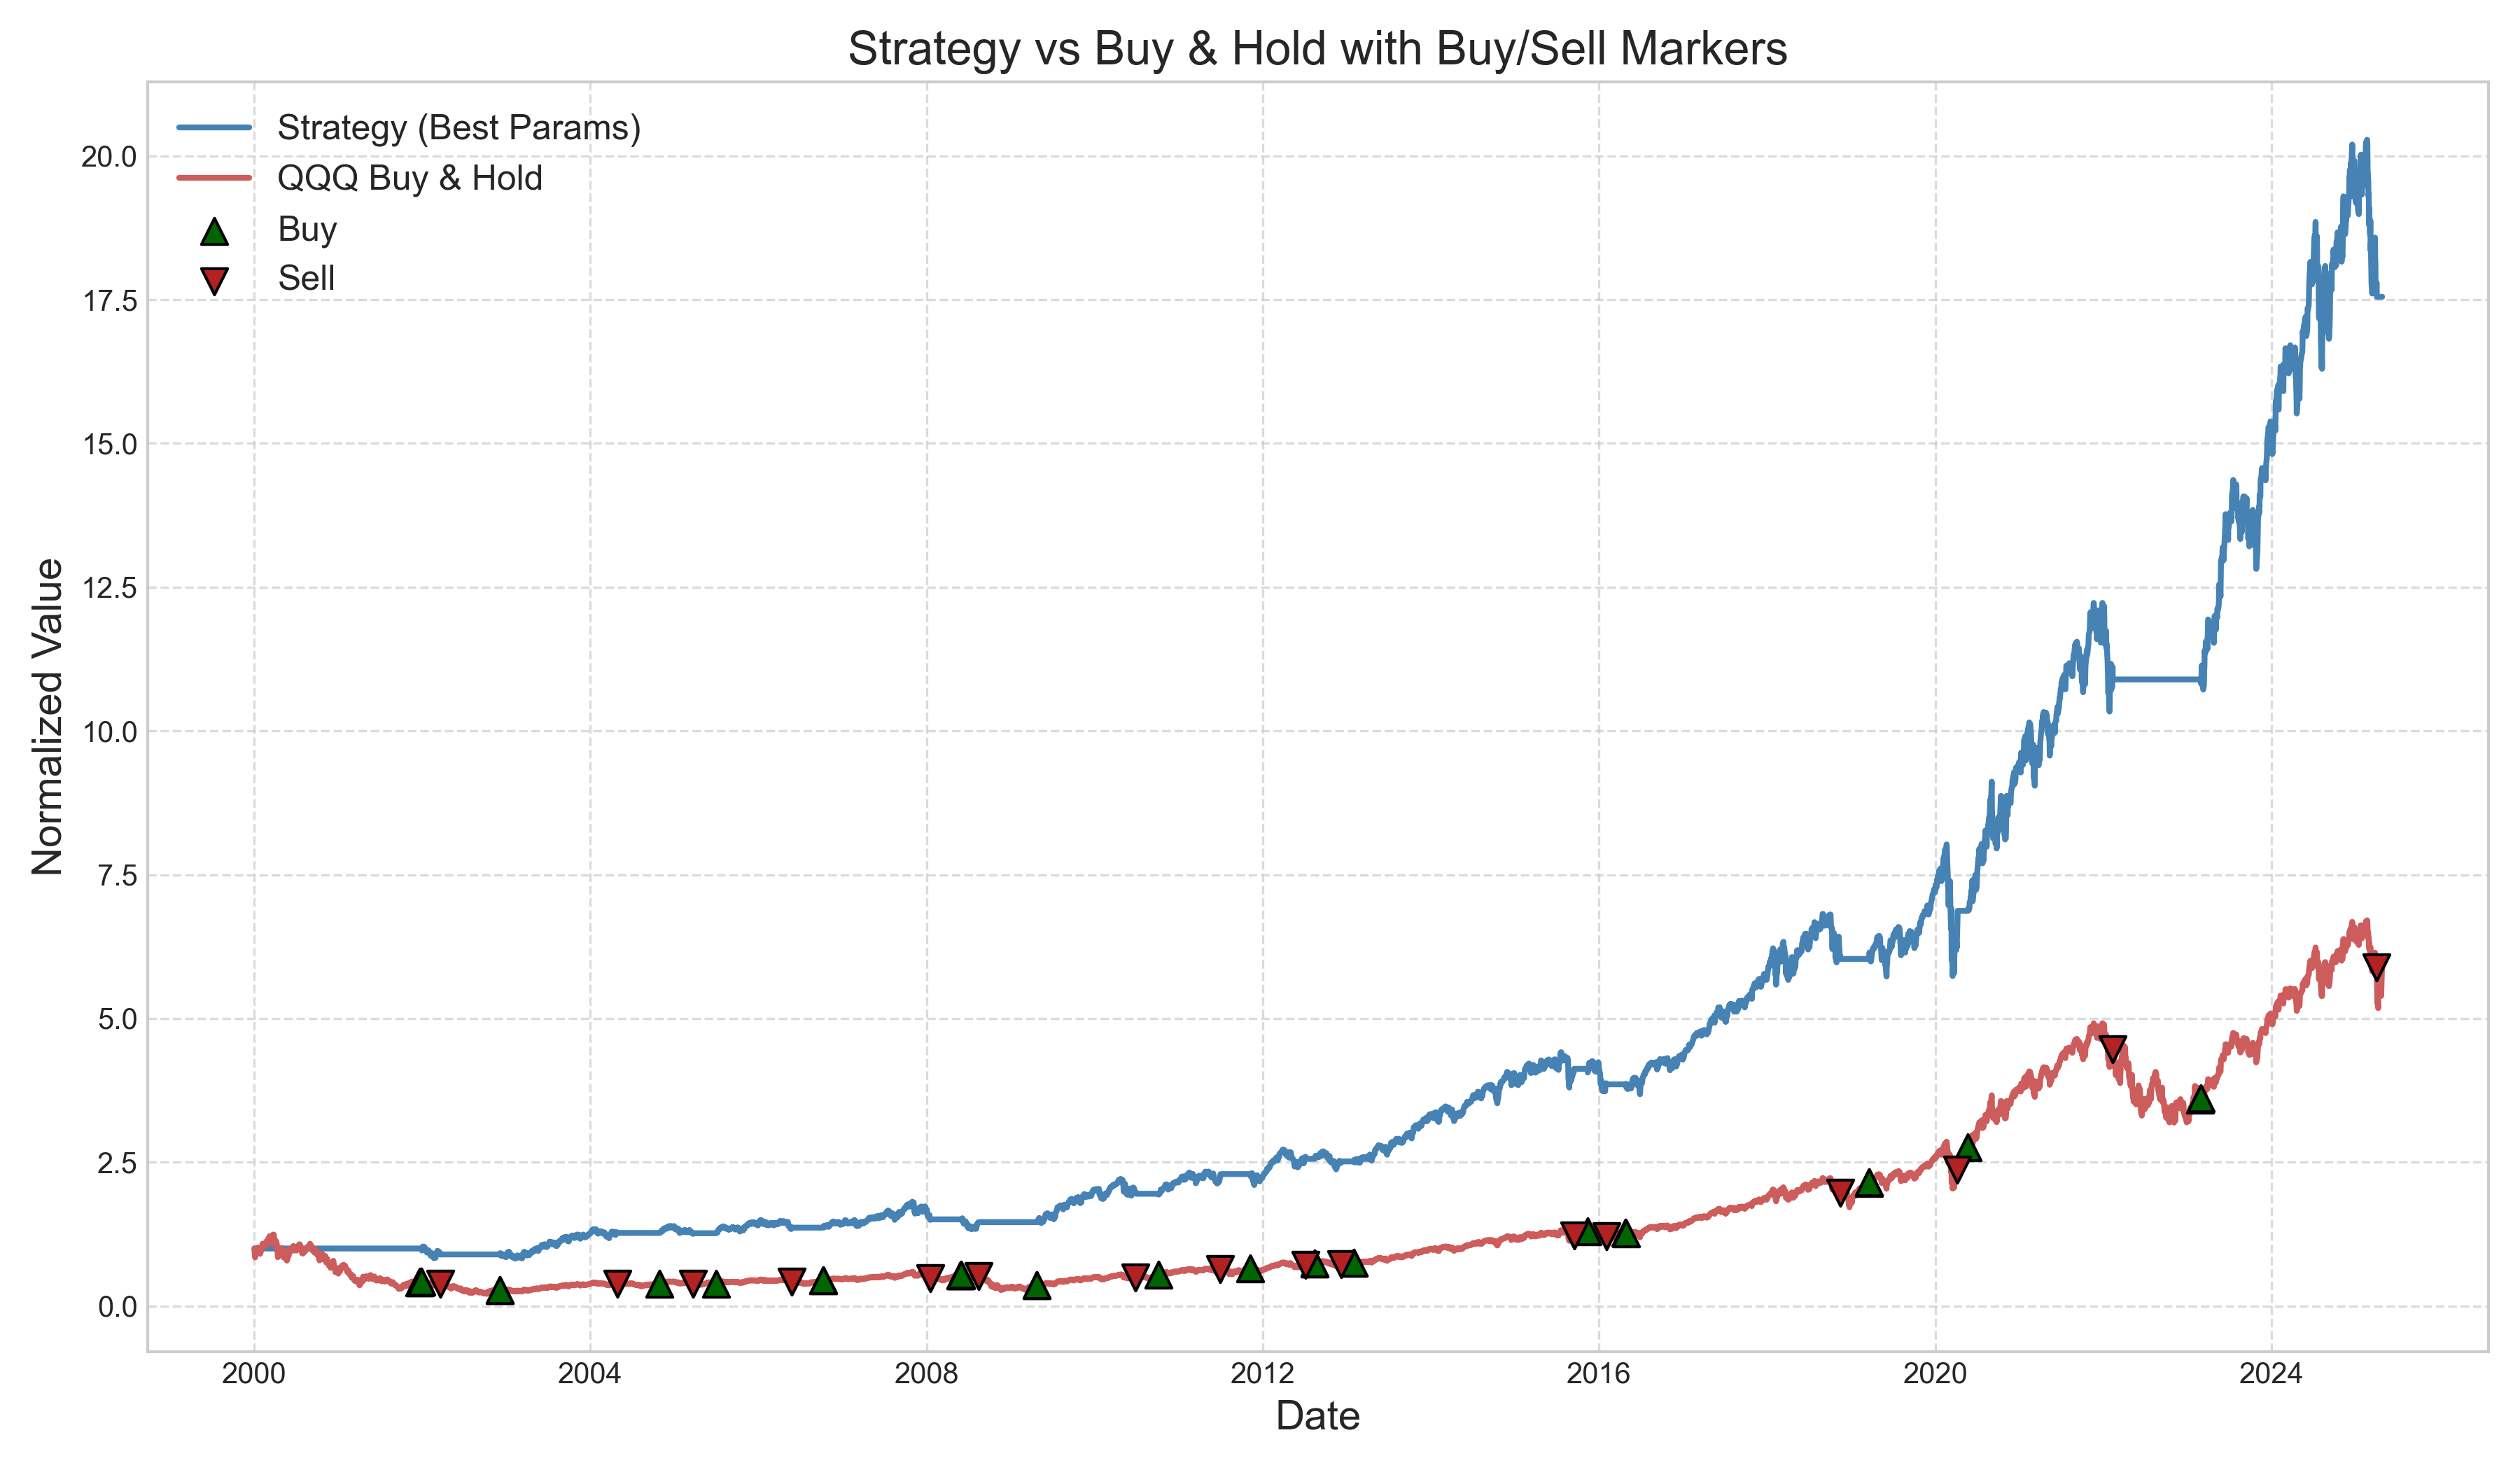
\includegraphics[width=\textwidth]{strategy_vs_buyhold_with_markers_QQQ_2000-01-01_to_2025-04-26.png}
    \caption{Figure 2 presents the log returns over time, emphasizing the volatility and distribution of returns in the dataset.}
    \label{fig:log_returns}
\end{figure}

Figure 1 highlights key crossover points between short-term and long-term moving averages, signaling potential trades. Figure 2 depicts the log returns over time, illustrating the volatility inherent in the dataset. Using the moving average crossover strategy, we achieved a return of 1655.00\%. However, this strong performance on a single index raises concerns about potential overfitting.

To provide further context, the moving average crossover strategy on the QQQ index achieved a total return of 1655.00\% over the period from 2000 to 2025, significantly outperforming the buy-and-hold return of 488.39\%. The best-performing configuration involved a short moving average window of 41 days and a long moving average window of 140 days, with an annualized Sharpe ratio of 0.79, indicating strong risk-adjusted returns. These results were generated using a custom backtesting framework built in Python, leveraging \texttt{backtrader} for simulation and \texttt{yfinance} for historical data retrieval. The codebase is designed for efficient parameter search with caching mechanisms to avoid redundant computations.




% --- Stock Selection and Filtering Section ---

\section{Stock Selection and Filtering}

To increase the generalizability and robustness of our model, we decided to expand our analysis from a single stock index (QQQ) to the broader S\&P 500 index. However, a key challenge was ensuring that all stocks in the S\&P 500 had sufficient data, particularly from January 1st, 2000, to avoid issues with incomplete historical data. 

The process involved:
\begin{itemize}
    \item Downloading the tickers for the S\&P 500 from Wikipedia.
    \item Filtering the tickers to only include those with data available since the start of 2000.
    \item Storing the tickers with sufficient data in a separate file for further analysis.
\end{itemize}

After filtering, we were left with a dataset of 353 stocks that met the data availability criteria. This step helps ensure that our models are not overfitting to stocks with missing or sparse data. The resulting list of stocks was then used in our backtesting process.

The list of tickers with sufficient historical data is stored in a separate file for future reference and to avoid re-fetching data in subsequent experiments.

\begin{figure}[h]
    \centering
    \includegraphics[width=\textwidth]{filtered_stocks_over_time.png}
    \caption{Figure 3: Stocks filtered to include only those with data available from January 1st, 2000, for the backtesting process. The final list of stocks was reduced to 353.}
    \label{fig:filtered_stocks}
\end{figure}

This selection process ensures that we can evaluate the robustness of trading strategies across a diverse set of stocks while minimizing data gaps.

\section{Discussion}
Currently, we are using technical indicators as our primary features because they are computationally efficient. We then apply a secondary layer of machine learning. However, solely relying on technical indicators can lead to overfitting, especially on a limited dataset like an index.

To move forward, we propose the following next steps:
\begin{enumerate}
    \item Apply our technical indicators and machine learning models across the entire S\&P 500 universe.
    \item Aggregate the performance results to measure consistency across different stocks.
    \item Generate additional features, such as volatility metrics, moving averages of volume, and relative strength indices.
    \item Implement ensemble methods that combine signals from multiple models and indicators.
    \item Use significance tests to validate whether observed returns are statistically meaningful.
    \item Explore adding fundamental features (e.g., P/E ratio, earnings growth) in future extensions of this work.
    \item This will also allow us to incorporate insights from asset pricing theory and broader financial principles, instead of purely relying on technical analysis.
\end{enumerate}
This will make our analysis more robust and allow for a better understanding of indicator generalizability across different stocks and market conditions.

yes 


\printbibliography


%%%%%%%%%%%%%%%%%%%%%%%%%%%%%%%%%%%%%%%%%%%%%%%%%%%%%%%%%%%%

\appendix

\section{Supplementary material} \label{app:info}

This stuff doesn't count towards your page limit.

\end{document}
